\documentclass[sigplan,nonacm]{acmart}
\settopmatter{printfolios=true}
\usepackage{graphicx} % Required for inserting images
\graphicspath{ {./images/} } %images subfolder
\usepackage[normalem]{ulem}

\title{Related Works}
\author{Mark Madler}
\begin{document}
\maketitle
%All are related to some degree -- so they are organized as follows:
\section{Related Works}
Generally all RDMA systems seek to optimize the use of underlying RDMA operations.
Different RDMA operations have different costs and benefits, for example one-sided verbs
are excellent at performing remote reads or other tasks which are not highly contentious. 
Depending on the application, some researchers opt to use two-sided sends while others
use one-sided writes. The advantage of using two-sided sends is that the remote CPU is 
involved and can handle highly contentious situations locally wihout the need for 
excessive RDMA communication. One-sided writes are generally more optimal when there 
is less contention as they avoid interaction with the remote CPU, but pose more of a challenge
when it comes to synchronization and contention.

% Distributed memory abstractiosn can generally be grouped into two categories: a Partitioned Global 
% Address Spaces (PGAS), and replicated address spaces. There exist multiple PGAS languages which allow 
% for programming of multiple machines in a more traditional shared memory style.

Distributed memory abstractions generally fall into a two categories:
Some global or Partitioned-Global Address Space (PGAS), and replicated address spaces. While both of these design philosophies 
generally rely on the same underlying verbs or at least some similar mechanisms they tend to 
serve different goals. The partitioned global address space model is great for creating a Distributed 
Shared Memory system (DSM), but lacks some of the performance that might be found in systems that support replication. 
A naiive PGAS model will incur large performance overheads if accessing remote data often
without concepts like caching or other methods to achieve data locality. Key-value stores on the other hand lack generality and can be used as shared memory, but 
either suffer from poor locality or high coherence overhead. Often times a performance optimization of key-value stores it to cache indexes for 
systems that have a complicated lookup process. Replicated Address space designs are very interesting as they do see the performance 
benefits of caching unlike a naiive pgas and some key-value stores, but they also see a performance drawback in terms of 
reduced memory size. Many concurrent data structures can easily be built upon these replicated address spaces, but these address 
spaces are not scalable. Of these models (distributed) key-value stores and PGAS models are more scalable. \textbf{Speculatively} our 
system will be much faster than existing optimized PGAS models because existing PGAS models have more expensive coherence 
between cached copies of data. This paper falls into the category of PGAS, but relies on the common programming practice 
to use Release Consistency, and the observation that the only time coherence is needed in Release Consistency 
is when there is a synchronizes-with edge between an acquire and a release.

distributed + pgas stuff:
farm (though there is replication for durability \cite{Dragojevic-NSDI-2014}), 

replicated stuff:
Kite (\cite{Gavrielatos-PPoPP-2020}), 

Distributed memory abstractions can generally be divided into three categories.
These categories are Key-value stores, DSMs, and other. The nomenclature surrounding 
these abstractions is generally not consistent across research and thus a definition of each 
of these categories follows. Key-value store are sometimes considered Distributed Shared Memory systems
since all memory accesses could be treated as hash-table lookups but this is not a holistic view. Key-value
stores are effective as databases and may lose performance if used as a DSM. Classic DSMs are a shared
memory abstraction which treats at least some portion of memory as globally addressable. These DSMs 
classically have some coherence protocol which allows for a consistent view of memory by all processes.
Maintaining this coherence is a bit more difficult than a system that is just a hashtable as communication is 
costly and caching should be implemented. Other 


%                       REPLICATED KVS
%------------------------------------------------------------------------------------
\section{KVS over RDMA}

    \subsection{Kite: efficient and available release consistency for the datacenter}
    This is the real entry paper. This is a replicated KVS over RDMA with a 
    "Linearizable variant of" \textbf{Release Consistency}. Some mention of Release Consistency
    as a "one sided barrier." Compares against Zookeeper and Derecho. Uses some 
    monotonically increasing clocks to track versions.\cite{Gavrielatos-PPoPP-2020} 

    \subsection{FaRM: Fast Remote Memory}
    Super similar to the entry paper in that is is a KVS for RDMA, but this one is I beleive disaggregated. 
    Farm could really be classified as a KVS or even a protocol. This design always replicates state info. 
    Provides \textbf{strict serializability}, so Transaction based consistency.
    So FaRM provides lock-free reads. The authors mention
    a "shared address space." \cite{Dragojevic-NSDI-2014}

    \subsection{FaRMv2: Fast General Distributed Transactions with Opacity}
    Just like FaRM but with opacity. Also providing \textbf{strict serializability}.
    Idk if this paper is really something to look at or not (TODO)\cite{Shamis-SIGMOD-2019}

    \subsection{HERD: Using RDMA efficiently for key-value services}
    Herd. Fast because it uses a weird combination of UD and message things.
    This combination is essentiall UC (unreliable connection) requests places 
    as writes to the server, then serviced by a server polling thread. The server replies over 
    UD (unreliable datagram) (this is a 2-sided send). One of the main ideas 
    of this paper is that writes can be faster than reads because there is 
    (at least with unreliable connection) no need for the destination to respond. 
    In the future it might be wise to refer back to this paper for info about the performance 
    metrics from RDMA verbs.\cite {Kalia-SIGCOMM-2014}

    \subsection{Sherman: A Write-Optimized Distributed B+Tree Index on Disaggregated Memory}
    This system is disaggregated meaning a system where compute and memory servers are separated. 
    Node-granularity. "consistent". Optimizations are established
    to target mainly chained atomic operations and write-amplification. Uses a cache of indexes to boost 
    performance, since they are just pointers it cannot have coherence problems. Introduce a 
    HOCL (Heirarchical On Chip Lock)\cite{Wang-SIGMOD-2022}

    \subsection{Using One-Sided RDMA Reads to Build a Fast, CPU-Efficient Key-Value Store (Pilaf) }
    Linearizable data store.  Self-veriftying meanin that they use checksum and size information stored along pointers
    that have been cached which ensures automatic garbage collection. Note that this paper has a great 
    analysis of IPoIB as well as RDMA vs verbs latency and thrup. This paper has 1 sided reads which are 
    initiated by the client while having store handled by the remote server. Uses Cuckoo hashing and uses 
    a reshuffling scheme where keys may move when all hash slots are full, but will always exist in at least 1 location.\cite{Mitchell-ATC-2013}

    
    \subsection{Scythe: A Low-Latency RDMA-enabled Distributed Transaction System for Disaggregate Memory }
    KVS again. Seeks to optimize concurrency control, timestamping, bandwidth. Uses Timestamp Oracle (TSO)
    hot-aware concurrecy control. Allows RPC. Basically split the design into two modes: low-heat and high-heat.
    Things like a Hot-aware takeout lock are used to ensure fairness. This whole system is very transactions focused. \cite{Lu-ACMtrans-2024}

    \subsection{HCL: Distributing Parallel Data Structures in Extreme Scales}
    Strictly serializabile KVS. HCL stands for Hermes Containder Library. This is essentially a library 
    which exports some high performance data structures and methods. Uses some RPC\cite{Devarajan-CLUSTER-2020}

    \subsection{BCL: A Cross-Platform Distributed Data Structures Library}
    Uses either MPI, OpenSHMEM, GASNET-EX, and UPC++ as backends. Uses a DSL to implement the data structures 
    exported by the library. \cite{Brock-ICPP-2019}
    
    \subsection{Rolex}
    Uses learned indexes. splits compute and memory. Referenced in newer papers as performing better than Sherman.
    Uses what they call "leaf-atomic shift sheme" to allow for new allocations. The one major performance drawback 
    is when retraining occurs (when data move out of the error range) The whole system must block for retraining. 
    This paper has lots of math and such describing their techniques. \cite{Li-FAST-2023}

    \subsection{Exploiting Hybrid Index Scheme for RDMA-based Key-Value Stores*** (Hstore)}
    Seeks to solve issue of range-lookups. Compares against Sherman and Clover beating both. 
    This does indeed outperform sherman on YCSB. Maybe problematic for LOCO. claims 54\% improvement 
    over sherman. Uses a hybrid scheme of skiplist and hashtable for range lookups and single lookups respectively.
    Uses a client / server model. GETs are one sided while other operations are two sided. supports "serializability"
    and there is come metion of writes being sequential. "strong consistency"\cite{Han-SYSTOR-2023}

    \subsection{Disaggregating Persistent Memory and Controlling Them Remotely: An Exploration of Passive Disaggregated Key-Value Stores}
    "Clover". Workes on Persistent memory. Uses interesting method of chaing updates together to avoid conflicts. Reads traverse
    these "chains" to find the latest write."shortcuts" are used and are issued in parallel to regualr reads, whichever 
    operation returns first is used. Wrtites occur out-of-place when does CAS pointer swing on the tail of the chain to the new data. also maybe faster 
    than Sherman but definitely not the fastest. the meta-data servers will handle the garbage collection when things are freed.\cite{Tsai-USENIX-2020}

    \subsection{AStore: Uniformed Adaptive Learned Index and Cache for RDMA-Enabled Key-Value Store}
    Supposedly outperforms \textbf{Sherman} by A LOT. ALso compares against "xstore" "Rolex" and "hybrid (not to be confused
    with the above hybrid index scheme which also independetly claims to be faster than Sherman)". 
    The results also suggest that Rolex outperforms \textbf{Sherman}. claims up to 91\% improvement over \textbf{Sherman}\cite{Qiao-IEEEtrans-2024}

    \subsection{Maintaining Cache Consistency in RDMA-based Distributed Key-Value storage System}
    note really worth considering it seems. This is indeed a KVS but only seems to compare against scale store. \cite{Hou-DSIT-2024}

    \subsection{FastStore: A High-Performance RDMA-Enabled Distributed Key-Value Store with Persistent Memory}
    not really worth considering. Again PM. COmpares against Clover and Sherman. Also is faster than Sherman with lower latency 
    as well as higher throughput. \cite{Xiong-ICDCS-2023}

    \subsection{LoLKV: The Logless, Linearizable, RDMA-based Key-Value Storage System}
    Weirdly does not compare against state of the art really. All of the comparisons are against older consensus protocols.
    LoLKV is worth looking at, but sincethere are no comparisons against Sherman I am more worried about the other papers 
    that do. It seems like this paper is more concerned about the consensus protocols. \cite{Alquraan-NSDI-2024}
%                       DSM OVER RDMA
%-----------------------------------------------------------------------------------
\section {DSM systems}

    \subsection{Scaling out NUMA-Aware Applications with RDMA-Based Distributed Shared Memory: MAGI}
    Page-based DSM. \textbf{Sequentially consistent} with the option of overriding in some cases. They use 
    smaller page sizes to try and over come page-based problems like write-amplification. They implement 
    strategies from traditional shared memory systems to enahnce their performance. They use specualtive 
    page faults to fetch pages before they are needed. Since the TLB is used extensively to maintain 
    a coherence within a node in terms of page visibility, there is a large overhead in the form of interrupts.
    The authors decided to batch these interrupts for improved performance. Unfortunately they have weak results
    which slow slight improvements over a "baseline" but do not compare against anything else. The baseline seems to be 
    their DSM without the speculation and batching.\cite{Hong-JCST-2019}

    \subsection{Efficient Distributed Memory Management with RDMA and Caching (GAM) }
    cache-line granularity DSM. Directory based, \textbf{Partial Store Order}. \textbf{PGAS addressing model}. 
    Use the directory to track the cache state at each node (DRMA cache). Attempsts to implement LRU 
    caching.  \cite{Cai-VLDB-2018}

    \subsection{Distributed Shared Object Memory}
    object based granularity, release consistency... too old for RDMA\cite{Guedes-WWOSIII-1993} %idk if worth reading

    \subsection{Gengar: An RDMA-based Distributed Hybrid Memory Pool}
    This is object based dsm over rdma but with non-volatile memory as well using Intel Optane. Seems to 
    also use this lease assignment idea like in \cite{Endo-IPDRM-2020} but is not page based. Uses a client / 
    server model where the servers provide DRAM and NVM to clients. The distributed DRAM is like a write-through 
    cache where the writes go through to Persistent memory. For some reason they provide longer leases 
    for hot objects (seems like this would increase worst case latency). Good results. \cite{Duan-ICDCS-2021}

    \subsection{TreadMarks: shared memory computing on networks of workstations}
    Was implemented over IP, lazy release consistency. Uses diffs to allow for multiple-writers. 
    Uses the page-size granularity, but diffs make this a little different. Also optimized for multiple threads
    on a local machine accessing the same page. \cite{Amza-Usenix-1994}

    \subsection{LITE Kernel RDMA Support for Datacenter Applications}
    This is page based DSM using the kernel. Has some care for permissions and security which is nice. 
    Claims to have more scalable thorughput than standard verbs. they run a DSM over their implementation.
    So this is not exactly a DSM but rather a way of using RDMA generally. \cite{Tsai-SOSP-2017}

    \subsection{MENPS: A Decentralized Distributed Shared Memory Exploiting RDMA} %% deep read this %%
        \begin{itemize}
            \item Page based DSM
            \item Special Diff merging and page sharing
            \item Combine write notices and logical leases (what is that?)\cite{Endo-IPDRM-2020}
        \end{itemize}

    \subsection{Argo DSM} 
    Page-based DSM. The authors propose a coherence trick where nodes will self-invalidate 
    or self-downgrade to avoid coherence traffic. They implement a message-free protocol (one sided verbs). 
    Built on top of MPI. Aim to resuce cost of directory based coherence. One of the main ideas is that 
    a node may read any data block as long as it will invalidate that data at the next synchronization point. \cite{Kaxiras-HPDC-2015}

    \subsection {GiantVM: A Novel Distributed Hypervisor for Resource Aggregation with DSM-aware Optimizations}
    Page-based DSM again but also works over TCP and RDMA. Basically its a distributed virtual CPU. It seems like 
    it is just a global address space that is known to the Hypervisor.\cite{Jia-ACO-2022}

    \subsection{Scalable RDMA performance in PGAS languages}
    This paper is for PGAS languages. Has an address hash table similar to LOCO for remote lookups. Written in 
    collaboration with IBM and details  the IBM XLUPC compiler + runtime. Some caching for performance. A little old of a paper
    so things like UPC++ were not around yet.\cite{Farreras-IPDPS-2009}

    \subsection {misc RDMA coherence papers}

    \subsection{Misc PGAS languages probably}
%-----------------------------------------------------------------------------------------
%                       PROTOCOLS OVER RDMA FOR CONSISTENCY
%----------------------------------------------------------------------------------------
\section{Protocols over RDMA for Consistency}

    \subsection{Notes on PGAS and "protocols"}
    It seems like there are not agreed upon semantics on what is a protocol. PGAS is a 
    memory model. For myself and posterity, PGAS is a memory model where the address space is logicaly partitioned across nodes.
    This means that there can be some reasoning about locality likely from virtual memory addresses.

    Some notes on MPI. MPI is a programming model which supports multiple communication backends. MPI 
    can run over IP, RDMA, etc. 

    \subsection {Odyssey: The Impact of Modern Hardware on Strongly-Consistent Replication Protocols}
    This paper is a summary of protocols used for RDMA communication. These protocols were used to 
    enforce consistency and were tested with a series of KVSs. This paper is related to Kite (same authors) 
    and Kite is one of the KVSs tested.\cite{Gavrielatos-EuroSys-2021}

    \subsection {Hermes: A Fast, Fault-Tolerant and Linearizable Replication Protocol}
    This paper \cite{Katsarakis-ASPLOS-2020} is one of the Protocols tested by the above paper Odyssey \cite{Gavrielatos-EuroSys-2021}. This 
    protocol guarantees linearizablity and is designed to work on replicated store systems.

    \subsection {Hamband: RDMA Replicated Data Types}
    This paper \cite{Houshmand-PLDI-2022} designed new RDMA data types that are replicated across nodes. This paper 
    is sort of a protocol paper as it implements this protocol to keep replicated data through either relaxed or 'strong consistency'.

    \subsection{Evaluation of RDMA opportunities in an Object-Oriented DSM}
    Interesting result is that it proves that invalidation protocols are better suited 
    for distributed systems. \cite{Veldema-LCPC-2007}
%----------------------------------------------------------------------------------------
%                       AWESOME TABLE
%----------------------------------------------------------------------------------------
\section{table i found}
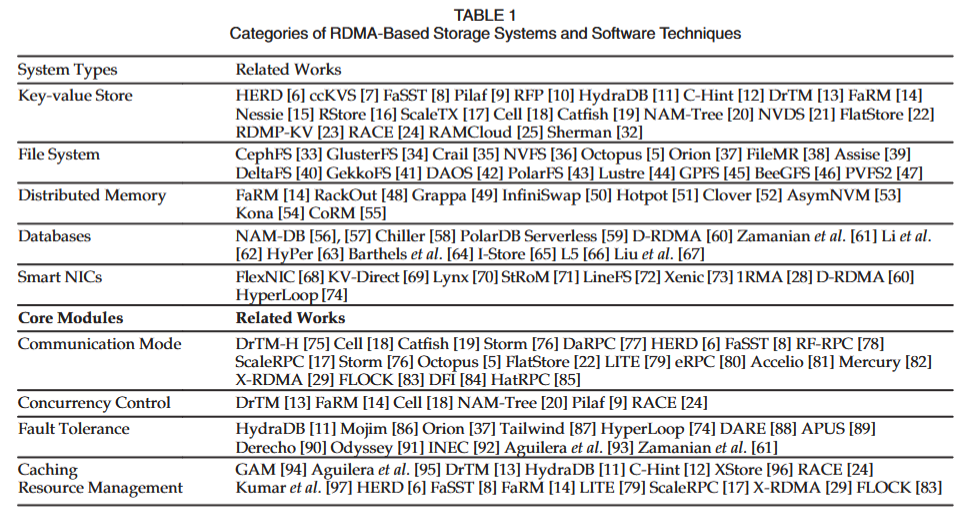
\includegraphics[width=0.5\textwidth]{Table_1_A_Survey_of_Storage_Systems_in_the_RDMA_Era}
\cite{Ma-PDS-2022}
%-----------------------------------------------------------------------------------------
%                       LOOSELY RELATED
%-----------------------------------------------------------------------------------------
%Loosely Related / Line of Work 
\section{Loosely Related but Evaluated}
    \subsection{CoRM: Compactable Remote Memory over RDMA}
    page based I think (re-read this)\cite{Taranov-ICMD-2021}

    \subsection{Rcmp: Reconstructing RDMA-Based Memory Disaggregation via CXL}
    page based and uses CXL, not comparable\cite{Wang-ACO-2024}
%-----------------------------------------------------------------------------------------


\bibliographystyle{acm}
\bibliography{relworks}
\end{document}